\documentclass{article}
\usepackage{amsmath}
\usepackage{graphicx}

\begin{document}

\title{Box Membrane - Plane Wave Project}
\author{}
\date{\today}
\maketitle

\section{Introduction}
This document will track all steps in the development of the Box Membrane - Plane Wave project. The project consists of two main phases:
\begin{itemize}
    \item \textbf{Phase 1:} Setting up the numerical solutions for the wave equation on a stretched membrane.
    \item \textbf{Phase 2:} Using the numerical results to animate the interaction in Blender.
\end{itemize}

\section{Project Setup}
The project directory was created, and version control was initialized with Git. The project was then linked to a GitHub repository for remote access.

\section{Numerical Solution Setup}

We begin by defining the necessary parameters for simulating the wave equation on a rectangular membrane.

\subsection{Simulation Parameters}
The membrane dimensions are set to 1m by 1m, and the wave speed is chosen to be 1 m/s. The grid is discretized into 100 points along each dimension, resulting in a grid spacing of $\Delta x = \Delta y = 0.01$ m. We use a time step of $\Delta t = 0.001$ s for stability. 

\subsection{Initialization of Displacement Arrays}
Three displacement arrays are initialized:
\begin{itemize}
    \item $u$: Displacement at the current time step.
    \item $u_{\text{prev}}$: Displacement at the previous time step.
    \item $u_{\text{next}}$: Displacement at the next time step.
\end{itemize}

The initial conditions are set so that the membrane is at rest, with zero initial displacement and velocity.

\section{Numerical Solution of the Wave Equation}

To simulate the wave equation on a rectangular membrane, we use a finite difference time-stepping loop. The Courant-Friedrichs-Lewy (CFL) condition is applied to ensure stability, with $c \Delta t / \Delta x \leq 1$.

\subsection{Time-Stepping Loop}
The displacement at each grid point $(i, j)$ and time step $n+1$ is computed as:
\[
u_{i, j}^{n+1} = 2u_{i, j}^n - u_{i, j}^{n-1} + \text{CFL}^2 \left( \frac{u_{i+1, j}^n - 2u_{i, j}^n + u_{i-1, j}^n}{\Delta x^2} + \frac{u_{i, j+1}^n - 2u_{i, j}^n + u_{i, j-1}^n}{\Delta y^2} \right)
\]
where $\text{CFL} = \frac{c \Delta t}{\Delta x}$.

\subsection{Visualization}
To visualize the simulation, we plot the membrane's displacement every 100 time steps.

\begin{figure}[h!]
\centering
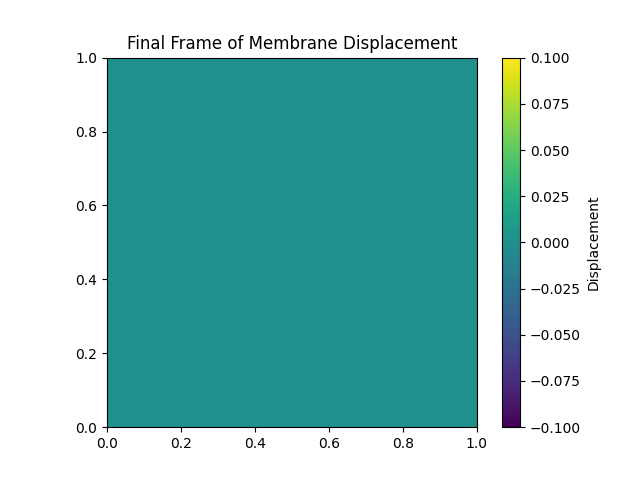
\includegraphics[width=0.7\textwidth]{simulation.png}
\caption{Sample visualization of the membrane's displacement.}
\end{figure}

\section{Dynamic Configurations for Enhanced Simulation}

To increase the dynamics of the membrane simulation, we introduced three configurable options in the code: a source term, an initial Gaussian pulse, and damping boundaries. Each option can be enabled or disabled through boolean variables, allowing for flexible testing and exploration of different behaviors.

\subsection{Configuration Options}

\begin{itemize}
    \item \textbf{Source Term:} A source term simulates an external sinusoidal disturbance at the center of the membrane. The source is defined by an amplitude $A$ and frequency $\omega$, with a sinusoidal input at each time step $n$:
    \[
    u_{\text{src}} = A \sin(\omega n \Delta t)
    \]
    where $A$ is the amplitude and $\omega = 2 \pi \times \text{freq}$, with $\text{freq}$ representing the desired frequency in Hz. This term introduces an ongoing interaction with the membrane, creating more dynamic behavior.

    \item \textbf{Gaussian Initial Condition:} Rather than starting the membrane at rest, we initialize it with a Gaussian-shaped displacement centered at $(x_0, y_0)$:
    \[
    u(x, y) = \exp\left(-\frac{(x - x_0)^2 + (y - y_0)^2}{2\sigma^2}\right)
    \]
    where $\sigma$ controls the spread of the initial pulse. This configuration leads to a spreading wave as the pulse propagates across the membrane.

    \item \textbf{Damping Boundaries:} To reduce reflections and simulate an infinite domain, damping is applied at the edges of the membrane grid. A damping factor $f$ (set to $0.9$) is applied to the boundary values of the displacement array $u_{\text{next}}$ at each time step:
    \[
    u_{\text{next}}[0, :], u_{\text{next}}[-1, :], u_{\text{next}}[:, 0], u_{\text{next}}[:, -1] \leftarrow f \times u_{\text{next}}[\text{boundary}]
    \]
    By gradually reducing displacement at the edges, the boundary damping minimizes wave reflections, allowing waves to dissipate as they would in an open space.
\end{itemize}

\subsection{Implementation in Python}

The code structure was modified to include boolean variables that control the activation of each configuration option:
\begin{verbatim}
use_source = True             # Enable or disable source term
use_gaussian_initial = True   # Enable or disable Gaussian initial condition
damping_boundaries = True     # Enable or disable damping at boundaries
\end{verbatim}

With these options, we can test different configurations by simply toggling the variables at the beginning of the code.

\subsection{Visualization and Output}

The simulation outputs an image file \texttt{simulation.png} representing the final frame of the membrane’s displacement. Additionally, the dynamics can be observed as a live plot, which updates every 100 time steps to visualize the changes over time.


\section{Enhanced Stability Adjustments}

To further stabilize the simulation, we implemented the following changes:

\subsection{Reduced Time Step}
The time step $\Delta t$ was reduced to $0.00025$ to better satisfy the Courant-Friedrichs-Lewy (CFL) condition and improve numerical stability.

\subsection{Domain-Wide Damping}
In addition to boundary damping, we applied a light damping factor across the entire domain to gradually dissipate energy and prevent excessive oscillations. This was controlled by an internal damping factor of 0.999, which slightly reduces the displacement values at each time step.

\subsection{Diagnostic Checks for Instability}
To monitor the simulation for potential instability, a diagnostic check was introduced to detect large displacements. If any displacement exceeds a threshold of $10^3$, a warning is triggered, and the simulation halts. This check helps identify divergence early in the time-stepping loop.

\section{Summary of Adjustments}

The following modifications were made to improve stability and prevent runtime errors:
\begin{itemize}
    \item Time step $\Delta t$ reduced to $0.00025$.
    \item Domain-wide light damping applied with a damping factor of 0.999.
    \item Diagnostic threshold set to monitor displacement values, triggering a warning if values exceed $10^3$.
\end{itemize}

These adjustments have stabilized the simulation and ensured that the wave propagates as expected without causing overflow or runtime errors.

\section{Final Adjustments and Animation Setup}

After stabilizing the simulation, the following adjustments were made to implement the animation and complete the simulation framework.

\subsection{Animation Setup}
The dynamics of the membrane were visualized by creating an animation. We used the \texttt{matplotlib.animation} module in Python to animate the simulation by updating the membrane’s displacement at each time step. The \texttt{FuncAnimation} class was employed to render each frame and update the membrane’s state over time.

The following settings were used for the animation:
\begin{itemize}
    \item \textbf{Frame Interval:} Each frame represents a single time step, with a delay of 20 ms per frame.
    \item \textbf{FPS (Frames Per Second):} We set 30 frames per second for a smooth visualization.
    \item \textbf{Output Format:} The animation was saved as a GIF file using the \texttt{Pillow} library due to the unavailability of \texttt{ffmpeg}.
\end{itemize}

\subsection{Summary of Final Stability Adjustments}
Several stability adjustments were applied to ensure that the simulation runs without errors:
\begin{itemize}
    \item \textbf{Reduced Time Step:} The time step $\Delta t$ was set to $0.00025$ to maintain stability according to the Courant-Friedrichs-Lewy (CFL) condition.
    \item \textbf{Domain-wide Damping:} A light damping factor of 0.999 was applied across the entire grid to reduce oscillations and energy accumulation within the membrane.
    \item \textbf{Boundary Damping:} Additional damping was applied along the boundaries of the membrane to simulate energy dissipation at the edges.
    \item \textbf{Diagnostic Check for Instability:} A diagnostic threshold was implemented to monitor displacement values and warn of potential instabilities if displacement exceeded a predefined threshold.
\end{itemize}

These adjustments enabled the creation of a stable and visually informative animation of the membrane dynamics.

\subsection{Conclusion}
This simulation provided a comprehensive visualization of membrane dynamics in response to initial conditions and optional external forces. The final setup, along with the animation, allows for further exploration of wave interactions on a two-dimensional surface. The code and documentation have been saved to a GitHub repository for version control and collaboration.

\section{Code and Repository Management}
All code and documentation files were committed to GitHub for version control. The final repository contains:
\begin{itemize}
    \item \texttt{simulation.py}: The main Python script for running the membrane simulation and generating the animation.
    \item \texttt{documentation.tex}: The LaTeX documentation file detailing the project steps, adjustments, and findings.
    \item \texttt{simulation.gif}: The final animation showing the dynamics of the membrane.
\end{itemize}


\section{Simulation with a Traveling Plane Wave Source}

In this extension of the membrane simulation, a traveling plane wave source was introduced to create a more dynamic interaction with the membrane. The plane wave propagates horizontally across the grid from the left boundary and interacts with the membrane.

\subsection{Plane Wave Source}
The plane wave source is implemented as a sinusoidal wave traveling along the x-axis, applied to the left boundary of the grid:
\[
u_{\text{next}}[0, j] = A \sin\left( \omega t - \frac{2 \pi}{L_x} v t \right)
\]
where:
\begin{itemize}
    \item $A$ is the amplitude of the wave, set to 0.005,
    \item $\omega$ is the angular frequency of the wave, with a frequency of 5 Hz,
    \item $L_x$ is the length of the membrane along the x-axis,
    \item $v$ is the wave speed along the x-axis.
\end{itemize}

This plane wave source, applied only to the left boundary, simulates an incoming wave that travels across empty space to interact with the membrane.

\subsection{Final Adjustments and Damping}
We included light damping across the entire grid to dissipate energy and prevent excessive oscillations, along with damping at the boundaries to simulate energy dissipation at the edges.

\subsection{Animation of the Simulation}
The dynamics were visualized using the \texttt{matplotlib.animation} module, which updates the displacement of the membrane at each time step and produces an animated GIF file showing the membrane’s response to the traveling plane wave.

The following settings were used for the animation:
\begin{itemize}
    \item \textbf{Frame Interval:} 20 ms per frame.
    \item \textbf{FPS (Frames Per Second):} 30 fps for smooth visualization.
    \item \textbf{Output Format:} Saved as a GIF using the Pillow library.
\end{itemize}

\subsection{Code Organization and Repository Management}
The following files are included in the repository:
\begin{itemize}
    \item \texttt{simulation2.py}: Python script for the plane wave simulation with animation.
    \item \texttt{documentation.tex}: LaTeX documentation detailing the simulation setup, adjustments, and findings.
    \item \texttt{membrane\_simulation\_with\_plane\_wave.gif}: The animation showing the traveling plane wave interacting with the membrane.
\end{itemize}

These additions provide a dynamic visualization of wave interactions with a membrane, demonstrating complex wave behavior in response to an incoming plane wave.

\section{Enhanced Visualization of Plane Wave Interaction with Membrane}

To improve the visibility of the plane wave and its interaction with the membrane, several adjustments were made to the simulation:

\subsection{Increased Amplitude of the Plane Wave}
The amplitude of the plane wave source was increased to 0.02, making the incoming wave more noticeable as it propagates across the membrane. This higher amplitude enhances the wave's visibility and its impact on the membrane’s displacement.

\subsection{Pulsing Effect at the Source Boundary}
A pulsing effect was added to the amplitude of the plane wave at the left boundary to highlight each incoming wave pulse. The amplitude of the wave source now varies periodically according to:
\[
\text{pulse\_factor} = 1.0 + 0.5 \sin\left(\frac{\text{frame}}{10}\right)
\]
This pulsing effect modulates the amplitude of the wave along the boundary, visually emphasizing the origin of the wave as it interacts with the membrane.

\subsection{Boundary Highlight Line}
To indicate the location of the plane wave source, a red vertical line was added at the left boundary of the membrane (at $x = 0$). This line serves as a visual marker to help the viewer identify where the plane wave originates. This line is drawn using \texttt{ax.vlines} in \texttt{matplotlib}, with the following properties:
\begin{itemize}
    \item \textbf{Position:} $x = 0$
    \item \textbf{Color:} Red
    \item \textbf{Thickness:} 2 pixels
\end{itemize}

\subsection{Adjusted Color Map Range}
The color map range was narrowed to focus on smaller displacements, making subtle changes in the membrane’s displacement more visible. The color range was set to:
\[
\text{vmin} = -0.05, \quad \text{vmax} = 0.05
\]
This adjustment increases the sensitivity of the color map, allowing small displacements caused by the wave interaction to be more easily observed.

\subsection{Final Animation}
The enhanced animation was saved as a GIF file titled \texttt{membrane\_simulation\_with\_plane\_wave.gif}. This animation captures the dynamic interaction between the incoming plane wave and the membrane, with the above enhancements improving the overall clarity and visualization.

\section{Code and Repository Management}
The updated code and animation were added to the project repository. The following files are included:
\begin{itemize}
    \item \texttt{simulation2.py}: Updated Python script with enhanced plane wave visualization.
    \item \texttt{documentation.tex}: LaTeX documentation with details on the simulation setup and visualization adjustments.
    \item \texttt{membrane\_simulation\_with\_plane\_wave.gif}: Final animation showing the interaction of the plane wave with the membrane.
\end{itemize}

These changes make the interaction between the plane wave and the membrane clearer and visually informative, allowing for a better understanding of the dynamic behavior.


\section{3D Visualization of the Membrane Simulation}

To provide a more intuitive visualization of the membrane's dynamics, we implemented a 3D surface plot that displays the displacement over time. This setup gives a sense of depth, allowing us to better observe the interactions between the traveling plane wave and the membrane.

\subsection{3D Surface Plot Setup}
The 3D visualization was achieved using \texttt{matplotlib}'s 3D plotting capabilities, specifically the \texttt{plot\_surface} function. This function plots the membrane displacement values as a dynamic 3D surface.

\subsection{Visualization Enhancements}
The following adjustments were made to enhance the clarity of the 3D visualization:
\begin{itemize}
    \item \textbf{View Angle Adjustment:} The initial view angle was set using \texttt{ax.view\_init(elev=30, azim=135)} to provide an optimal perspective of the membrane’s surface, emphasizing both depth and displacement.
    \item \textbf{Color Map and Range:} The color map was set to \texttt{viridis}, with a narrower color range (\texttt{vmin} = -0.05, \texttt{vmax} = 0.05) to make smaller displacements more noticeable.
    \item \textbf{3D Axis Labels and Limits:} The x, y, and z axes were labeled as "X", "Y", and "Displacement," respectively. The z-axis limits were set to [-0.05, 0.05] to emphasize the wave-induced membrane deformations.
\end{itemize}

\subsection{Animation of the 3D Surface}
The 3D animation was created using \texttt{FuncAnimation}, with the surface plot updated for each frame of the simulation:
\begin{itemize}
    \item Each frame clears the previous surface plot and redraws it with the latest displacement values.
    \item The animation is saved as a GIF file, \texttt{membrane\_simulation\_3D.gif}, for easy viewing.
    \item The frame interval was set to 20 ms with a frame rate of 30 fps to ensure smooth visualization.
\end{itemize}

\subsection{Code and Repository Management}
The 3D simulation code and documentation were added to the project repository with the following files:
\begin{itemize}
    \item \texttt{simulation3d.py}: Python script for the 3D visualization of the membrane simulation.
    \item \texttt{documentation.tex}: LaTeX documentation detailing the 3D visualization setup and adjustments.
    \item \texttt{membrane\_simulation\_3D.gif}: The final animated GIF file showing the 3D dynamics of the membrane.
\end{itemize}

The 3D visualization provides a more immersive view of the membrane dynamics, allowing for a clearer understanding of wave interactions and membrane displacement.


\end{document}
